
%%%%%%%%%%%%%%%%%%%%%%%%%%%%%%%%%%%%%%%%%%%%%%%%%%%%%%%%%%%%%%%%%%%%%
%%%
%%% Set these variables appropriately
%%%
\newcommand{\AUTHORS}{Kevin Lee, Akshay Mittal, Sachin Ravi \\ \textit{Department of Computer Science} \\ \textit{Princeton University} \\}
\newcommand{\TITLE}{Adaptive Data Placement in NewSQL Systems}
\newcommand{\KEYWORDS}{NewSQL, colocation, SQLFire}
\newcommand{\CONFERENCE}{}
\newcommand{\PAGENUMBERS}{yes}       % "yes" or "no"
\newcommand{\TOAPPEAR}{no}
%%%
%%%
%%%%%%%%%%%%%%%%%%%%%%%%%%%%%%%%%%%%%%%%%%%%%%%%%%%%%%%%%%%%%%%%%%%%%

%%%% Setup the document/page
\documentclass[pdftex,twoside,twocolumn,10pt,letterpaper]{article}
\usepackage{ifthen}

\ifthenelse{\equal{\PAGENUMBERS}{yes}}{%
\usepackage[nohead,
            left=1in,right=1in,top=1in,
            footskip=0.5in,bottom=0.75in     % Room for page numbers
            ]{geometry}
}{%
\usepackage[noheadfoot,columnsep=0.2in,
            margin=1in,centering,truedimen]{geometry}
}

\usepackage{fancyhdr}
\usepackage[numbers,sort]{natbib}
\usepackage{xspace}
\usepackage{booktabs}
\usepackage{subfig}
\usepackage[T1]{fontenc}
\usepackage{textcomp}
\usepackage{mathptmx}   % Times + Times-like math symbols
\usepackage{courier}
\usepackage[scaled=0.92]{helvet}
\usepackage{amsmath}

\usepackage{color}
\usepackage[pdftex]{graphicx}
\ifthenelse{\isundefined{\wantBW}}{%
  \usepackage[colorlinks]{hyperref}%        % for online version
}{%
  \usepackage[pdfborder={0 0 0}]{hyperref}% % for paper (B&W) version
}
\newcommand{\URL}[1]{\url{#1}}

%%%%% Setup for PDF
\hypersetup{%
pdfauthor = {\AUTHORS},
pdftitle = {\TITLE},
pdfsubject = {\CONFERENCE},
pdfkeywords = {\KEYWORDS},
bookmarksopen = {true}
}

%\setlength{\parindent}{0pt}
%\setlength{\parskip}{0pt}
\renewcommand{\headrulewidth}{0pt}
\newcommand{\Paragraph}[1]{\vspace{-2ex}\paragraph{#1.}}
\setlength{\topmargin}{-.15in}

\ifthenelse{\equal{\PAGENUMBERS}{yes}}{%
  \pagestyle{plain}
}{%
  \pagestyle{empty}
}

\newcommand{\acks}{\section*{Acknowledgments}}

\makeatletter\long\def\@makecaption#1#2{
   \vskip 10pt
   \setbox\@tempboxa\hbox{\textsf{#1: #2}}
   \ifdim \wd\@tempboxa >\hsize % IF longer than one line:
       \textsf{#1: #2}\par      % THEN set as ordinary paragraph.
     \else                      % ELSE  center.
       \hbox to\hsize{\hfil\box\@tempboxa\hfil}
   \fi}
\makeatother

\clubpenalty=10000  % Don't allow orphans
\widowpenalty=10000 % Don't allow widows

\usepackage{titlesec}

\titlespacing\section{0pt}{5pt plus 2pt minus 2pt}{0pt plus 2pt minus 2pt}
\titlespacing\subsection{0pt}{4pt plus 2pt minus 3pt}{2pt plus 1pt minus 3pt}
\titlespacing\subsubsection{0pt}{4pt plus 2pt minus 2pt}{0pt plus 2pt minus 3pt}

%\usepackage{biblatex}

%%%%%%%%%%%%%%%%%%%%%%%%%%%%%%%%%
\usepackage{float}
\setlength{\textfloatsep}{2pt plus 2pt minus 2pt}
%\addtolength{\abovecaptionskip}{-2cm}
%\setlength{\belowcaptionskip}{-15pt}
%\setlength{\intextsep}{0pt plus 2pt}
%%%%%%%%%%%%%%%%%%%%%%%%%%%%%%%%%

\title{\textbf{\TITLE}}
\author{\AUTHORS}
\date{}

% Compact itemize and enumerate.  Note that they use the same counters and
% symbols as the usual itemize and enumerate environments.
\def\compactify{\itemsep=0pt \topsep=0pt \partopsep=0pt \parsep=0pt}
\let\latexusecounter=\usecounter
\newenvironment{CompactItemize}
  {\def\usecounter{\compactify\latexusecounter}
   \begin{itemize}}
  {\end{itemize}\let\usecounter=\latexusecounter}
\newenvironment{CompactEnumerate}
  {\def\usecounter{\compactify\latexusecounter}
   \begin{enumerate}}
  {\end{enumerate}\let\usecounter=\latexusecounter}

\newcommand{\comment}[1]{}
%\newcommand{\comment}[1]{\textcolor{red}{#1}}
\newcommand{\ignore}[1]{}

\newcommand{\xc}[1]{\mbox{\textit{#1}}}
\newcommand{\la}{\leftarrow}
\newcommand{\ra}{\rightarrow}
\newcommand{\somespace}{\hspace{0.1cm}}

\def\discretionaryslash{\discretionary{/}{}{/}}
\def\discretionarydot{\discretionary{.}{}{.}}
\def\discretionarycolon{\discretionary{:}{}{:}}
{\catcode`\/\active
\catcode`\.\active
\catcode`\:\active
\gdef\URLprepare{\catcode`\/\active\let/\discretionaryslash
                 \catcode`\.\active\let.\discretionarydot
                 \catcode`\:\active\let:\discretionarycolon
        \def~{\char`\~}}}%
\def\URL{\bgroup\URLprepare\realURL}%
\def\realURL#1{\tt #1\egroup}%

\newcommand{\eg}{{\em e.g.}, }
\newcommand{\ie}{{\em i.e.}, }
\newcommand{\etal}{{\em et al.\ }}

\def\check{\stackrel{{\scriptscriptstyle ?}}{=}}

\setlength{\bibsep}{0pt plus .5pt minus .25pt}

\begin{document}
\maketitle

% -*-LaTeX-*-
% $Id: abstract.tex 70 2007-01-30 21:59:16Z nicolosi $

\begin{abstract}
In this paper we present a method for configuring the placement of data onto servers in NewSQL systems to minimize the cost of executing a known query workload.  Mainly, we apply ideas from database literature on optimal view materialization to colocate related data necessary for executing important joins within the memory of each data server. Through experiments in Emulab using SQLFire, we show that using our method to determine data placement configurations allows for adaptivity and improved performance with query workloads when compared to other data placement strategies.
\end{abstract}   
\section{Introduction}
\label{sec:intro}

NewSQL storage options such as MemSQL and SQLFire are gaining traction in industry because traditional RDBMS struggle with the scale associated with web services.  These NewSQL distributed storage services allow one to horizontally scale by adding more commodity machines as necessary without giving up strong transactional and consistency requirements as many NoSQL storage services do.  Though there exist many NewSQL options, all offering different internal architectures, we concentrate our efforts on in-memory databases that allow one to configure the placement of data across data servers through partitioning and replication, such as VMWare's vFabric SQLFire.

Depending on the placement of data in such NewSQL systems, the time required to execute a given query workload can vary greatly.  When considering the optimal data placement to handle a given query workload, the main nontrivial goal is to colocate related data necessary for the execution of important joins onto each data server.  Each data server can then execute an assigned portion of such important joins through only having to use the colocated data stored in its own memory.  However, if the data placement is configured poorly, many important joins may require gathering missing data from other data servers.  Such distributed joins can be very expensive to perform and are generally not supported.

The optimality of a data placement configuration for a NewSQL system is thus highly dependent on the query workload to be handled.  This presents key technical challenges as a developer must be able to analyze a query workload to understand which joins are important and do a complicated cost-benefit analysis to determine how to place the data.  We present an automated method for doing such an analysis, when given a data model and a query workload, to produce an optimal data placement configuration onto a set of servers.  We evaluate our method using an Emulab environment using SQLFire and the TPC-H query workload and find our method is able to adapt to varying query workloads to produce highly optimized data placement configuration when compared to other strategies.
\section{Background}
\label{sec:background}
We focus on NewSQL systems that allow one to manually determine the placement of data on servers in the system.  Specifically, we use VMWare's vFabric SQLFire 1.0~\cite{web:sqlfire} as the distributed database for holding the tables and serving the queries in our research. It is an in-memory distributed NewSQL database that provides scalability and high performance for large workloads. Its memory-optimized architecture minimizes the disk I/O time which is the main performance bottleneck in traditional databases.

In NewSQL systems like SQLFire, one can assign servers to one or more server groups.  Server groups are in charge of storing the data for a given set of tables.  Tables must either be partitioned~\cite{web:paritioning} or replicated~\cite{web:replication} across the servers of the group, but not both.

Partitioning a table distributes the rows of the table across the server group based on values of a specified partitioning column through hash-partitioning.  Furthermore, if two tables $s$ and $t$ are partitioned on the same column, one can specify that the partitions of $t$ be colocated with the partitions of $s$.  Doing so will distribute $s$ onto servers and then additionally colocate rows of $t$ with matching values for the partitioning column onto the same servers.  A server storing partitions can only execute a join between partitions if one is specified to be colocated with the other.

Replicating a table in a server group creates a synchronous replica of the entire table in each server of the group.  There is no limitation on the joins a server can do between replicated tables and other replicated tables or partitions.  Queries from a client to the system are broken and distributed so that each server handles the portion of the query that it can answer using its own data.  The results to the query are then combined and returned to the client.
\section{Design}
\label{sec:design}
We design a method for producing data placement configurations in NewSQL systems with tables partitioned and replicated in a manner to optimally colocate data with respect to a given query workload.  We look to previous database literature on automatically selecting materialized views for SQL databases. In many ways, selecting an optimal view to materialize is similar to selecting related table data to colocate as both involve finding and taking action on the most interesting table relationships with respect to a query workload.

\subsection{Estimating Colocation Benefits}
We first need to be able to quantify the benefit gained from colocating two tables.  For the view materialization problem in \cite{Yang:1997}, when considering a candidate view for materialization $V$, the query processing cost $C(Q,V)$ of a query workload $Q$ when using $V$ as the only view is examined.  With $S$ as the set of queries in $Q$, $q$ as a query in $S$, and $f_q$ as the frequency of $q$ in $Q$, this processing cost is intuitively:
\vspace*{-8pt}
\begin{equation}
C(Q,V) = \sum_{q \in S}f_qC(q,V)
\vspace*{-8pt}
\end{equation}
We reapply this equation to find the cost of a workload for a server when tables $s$ and $t$ are colocated in its memory as:
\begin{equation}
C(Q,s,t) = \sum_{q \in S}f_qC(q,s,t)
\vspace*{-5pt}
\end{equation}
This is essentially the cost of $Q$ when joins between $s$ and $t$ can be done locally on the server.  We also define $C(Q)$ to be the query processing cost of $Q$ for the server when it is never the case that the two tables required for any join are colocated in memory.  We define a distributed join to be a join where a server must fetch involved tables from different servers of the system for the join to be executed.  $C(Q)$ is thus the cost of executing $Q$ when all joins are distributed. The benefit of colocating $s$ and $t$ is thus:
\vspace*{-6pt}
\begin{equation}
Benefit(Q,s,t) = C(Q) - C(Q,s,t)
\vspace*{-8pt}
\end{equation}
We calculate $C(q,s,t)$, for any query $q$, based on our own heuristic cost model that estimates the number of row accesses required to perform the distributed joins of $q$. Only joins between tables from $\{s,t\}$ comes at no cost.  For each distributed join, we count the number of row accesses done to fetch both tables involved and perform the join.  For the purposes of our model, we assume that a server must even fetch $s$ or $t$ if they are in a join with a table that is not from $\{s,t\}$.  We also assume the join is performed by scanning one table for each row of the other table.  For a query with distributed joins between any tables $A$, with $|A|_r$ rows, and $B$, with $|B|_r$ rows, and $s$ and $t$ colocated, we thus assign a cost of:
\vspace*{-4pt}
\begin{equation}
\label{eq:cost}
C(q,s,t) = \sum_{A\bowtie B\in q\mid A\notin \{s,t\} \lor B\notin\{s,t\}}|A|_r + |B|_r + |A|_r|B|_r
\vspace*{-4pt}
\end{equation}
\noindent This involves one access per row of both tables in order to fetch both tables and the product of the number of rows of both tables in order to execute the join.

\subsection{Partitioning}
We next decide how to optimally partition the data in a manner that avoids expensive distributed joins.  To do this, we define a weighted graph $G = (V,E)$ to represent the table relationships in the data model. Each node $v \in V$ represents a table in the data model. A directed edge $e = (u,v) \in E$ represents a foreign key relationship where $u$ is the "parent" table with the referenced key and $v$ is the "child" table with the foreign key. 
%The cost of an edge $c(e)$ is the cost to complete the query workload assuming that the two tables exists in the same server, or $C(Q,u,v)$.%
Let $DirectedBenefit(Q,s,t)$ be the same as $Benefit(Q,s,t)$ except that the benefit of colocation is only gained when $s$ is the parent and $t$ is the child of the join.  We then assign a weight to the edge $(u,v)$ equal to $DirectedBenefit(Q,u,v)$.  We refer the reader to Figure~\ref{fig:schema} for an example of what this graph looks like for the TPC-H schema.

Using $G$, we pick the $k$ best nodes (tables) to serve as partition "centers", meaning that we will pick the partitioning columns from these $k$ tables. To decide which tables are the $k$ best nodes to serve as partition centers, we define a benefit function $r_c$ which quantifies how useful a table would be if we picked a partitioning column from that table.
%Let $DirectedBenefit(Q,s,t)$ be the same as $Benefit(Q,s,t)$ except that the benefit of a join is only gained when $s$ is the parent and $t$ is the child.%
The function is defined as the sum of the weights of its outgoing edges added to the size of the table:
\vspace*{-8pt}
\begin{equation}
r_c(u) = \left( \sum_{e = (u,v)} DirectedBenefit(Q,u,v) \right) + |u|.
\vspace*{-7pt}
\end{equation}

The first part of the expression quantifies the benefit of colocating partitions of "child" tables with $u$, and the second part represents the fact that we generally want to partition larger tables. 

We pick the partition "centers" in an iterative process. We pick the node with the highest $r_c$ value and then remove this node and the nodes it was connected to in the graph. We then recompute $r_c$ for all the remaining nodes in the graph and iterate by picking the node with the highest value again until we have picked $k$ nodes.

Having picked these "centers", we then greedily assign other tables to partition and be colocated with them by assigning each table to the "center" for which its join on the partitioning column gives the most benefit.  We note that greedily assigning a table to a "center" may result in poor configurations in the case that the table has many important joins with tables that are not "centers".  We thus consider upgrading such tables to replicated tables in a later step.  If $S$ is the set of centers, a table $u$ is assigned to the center $A(u)$ as defined by:
\vspace*{-6pt}
\begin{equation}
A(u) = \max_{c \in S} \{DirectedBenefit(Q, c, u)\}
\vspace*{-6pt}
\end{equation}
Each "center" and its assigned tables make up what we call an entity group. An entity group is a unit for a set of tables that are all colocated and stored in the same server group.  If a table cannot be joined with any "center" on the partitioning key, it becomes a candidate for replication.

\begin{figure}
\centering
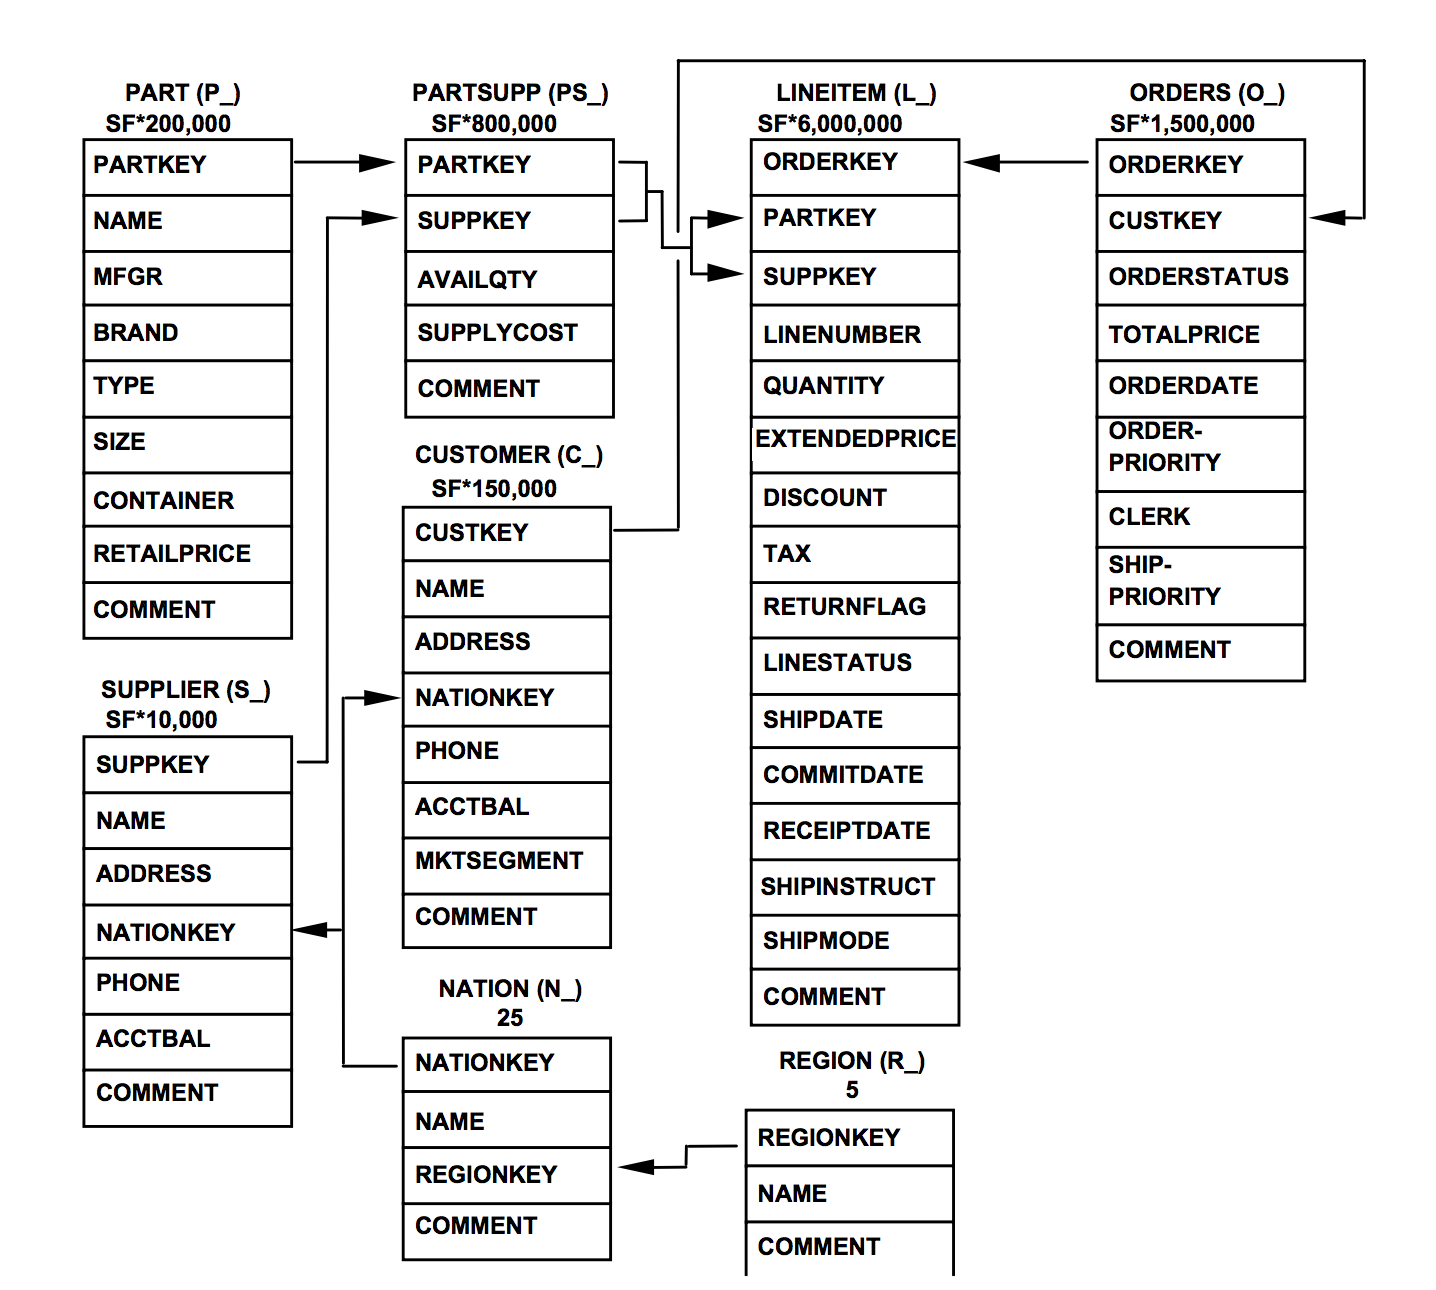
\includegraphics[scale=0.3]{TPC-H_DataModel.png}
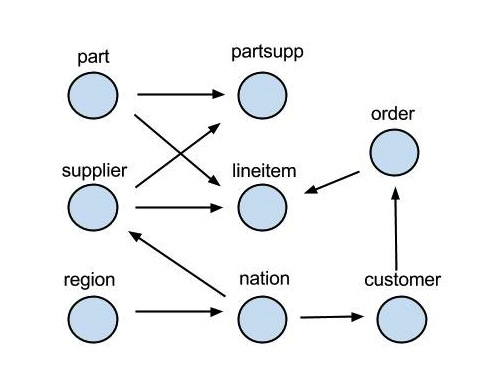
\includegraphics[scale=0.25]{ForeignJoinGraph.jpg}
\caption{\footnotesize{TPC-H Schema and corresponding graph produced without edge weights.}}
\label{fig:schema}
\end{figure}

\subsection{Replication}
In the next step, we decide which tables to pick to replicate in the system. The tables we consider for replication are those that are not partition centers.  Similar to with partitioning, we pick the $m$ best pairings of tables and entity groups to replicate into by defining a replication benefit function $r_r$, for each candidate table $u$ and entity group $E$. 

For each entity group $E$, given the average server memory size $\beta$, we can approximate the number of servers necessary to store $E$. Assuming $|P|$ is the sum of the sizes of the tables to be partitioned in $E$, we say this is 
\vspace*{-4pt}
\begin{equation}
\label{eq:numServers}
n = \lceil \frac{|P|}{\beta} \rceil
\vspace*{-4pt}
\end{equation}

Additionally, let $\phi(u)$ be the update rate of table $u$. The function $r_r$ quantifies the benefit of replicating table $u$ into the existing entity group $E$ as

\begin{equation}
\vspace*{-6pt}
r_r(u, E) = (\sum_{t \in E} Benefit(Q,t,u)) - |u| \cdot n - |u| \cdot \phi(u) \cdot n
\vspace*{-2pt}
\end{equation}

The first expression in the equation represents the benefit of colocating the replicated table in the entity group by enumerating the benefit gained by being able to do joins with $u$ and the tables in $E$ locally. The last two expressions in the equation represent the cost of colocating the replicated table by enumerating the cost to store the table at each server and the cost to send each update to the table synchronously to each server.  We rank the candidates by $r_r$ and then add the top $m$ replication candidates to the corresponding entity groups.  If a chosen replication candidate was partitioned and colocated with an entity "center" in the previous step, we override this decision and choose to replicate the table into one or more entity groups instead.

% This part can be cut based on how useful it is in the evaluation
\subsection{Server Assignment}
We now have entity groups containing an entity "center" and colocated partitions and replicated tables. In the last step, we consider assigning entity groups to a number of servers to form a server group.

Given the average server size, we can reuse Equation \ref{eq:numServers} to find the minimum number of servers needed to store an entity group $E$ while accounting for the space needed by the replicated tables in $E$. However, there is the question of how many servers to dedicate to $E$ beyond this minimum amount so that performance is optimal.

We do a cost-benefit analysis to determine how many servers to add beyond the minimum amount. Suppose the amount of servers assigned to $E$ is $n$; in the first iteration, $n$ is the minimum number of servers required. $m(n, E) = \frac{|P|}{n} + |R|$ gives the memory consumed by $E$ for a server when $E$ uses a server group of $n$ servers, $|P|$ is the sum of the sizes of the tables to be partitioned in $E$, and $|R|$ is the sum of the sizes of the replicated tables in $E$.  

With $\phi(R)$ as the average update rate of the tables in $R$, we repeatedly add a server to the group if 
\vspace*{-4pt}
{\small
\begin{equation}
b(n,E) = (m(n,E) - m(n+1,E)) - |R| - \phi(R) \cdot |R| > 0
\end{equation}
}
where $b(n,E)$ quantifies the point at which the cost of adding a server is greater than the benefit the extra server provides. The first part of the equation is the benefit of adding an additional server, as it represents the space savings a server gets through adding one more server to the group. The second part of the equation represents the cost of adding one more server due to additional replication and synchronous updates required.

We also accept a maximum number of servers parameter and stop adding servers to a server group before this parameter is exceeded.  Once a mapping of entity groups to server groups is produced, we leave it to the developer to map the server groups onto actual physical servers.

% \begin{figure}
% \centering
% \includegraphics[scale=0.50]{Flexible_Parallel.png}
% \caption{Flexible Parallel}
% \label{fig:flexible_parallel}
% \end{figure}

\section{Evaluation}
\label{sec:eval}
We build a Java-based tool~\cite{web:githublink} that takes a data schema, a query workload, a number of servers, and an average server memory size and implements our method to automatically produce a data placement configuration.  For now, we require the developer to hand-tune $k$, the number of entity centers, and $m$, the number of pairs of replicated tables and entity groups.  We look to automatically choosing $k$ and $m$ in future work. The results in our experiments use $k=2$ and $m$ as just high enough so that all tables are in a server group.  

\subsection{Benchmark}
\label{sec:benchmark}
We leverage the TPC-H benchmark~\cite{web:tpch} to test the configurations produced by our tool. The benchmark was designed for business applications' query testing purposes. It provides a table schema which has a combination of foreign keys and queries that have varying level of complex joins.

The script \texttt{dbgen} from the TPC-H specification takes in a scaling factor when generating the tables of our choice. By default, it generates all the tables as shown in Figure~\ref{fig:schema}. The scaling factor of 1 generates 1GB dataset which includes all the tables shown in Table~\ref{tab:dataset1gb}.

\comment{
\begin{figure}[!ht]
    \centering
    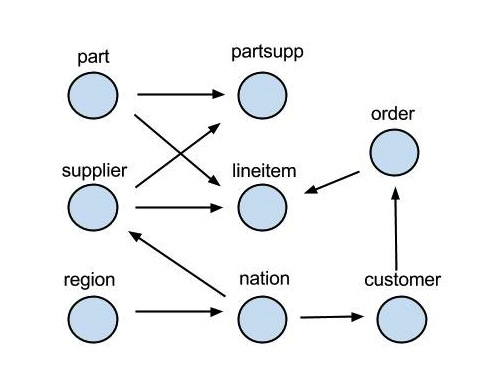
\includegraphics[scale=0.2]{ForeignJoinGraph.jpg}
    \qquad
    \resizebox{3.5cm}{!}{
\begin{tabular}{|c||c|}
\hline
\textbf{Table Name} & \textbf{Number of Rows}\\
\hline
customer & 150 K\\
\hline
lineitem & 6000 K\\ % 6001215
\hline
nation & 25\\
\hline
orders & 1500 K\\
\hline
partsupp & 800 K\\
\hline
part & 200 K\\
\hline
region & 5\\
\hline
supplier & 10 K\\
\hline
\end{tabular}
}
\comment{
    \begin{tabular}[b]{cc}\hline
      Table head & Table head \\ \hline
      Some values & Some values \\
      Some values & Some values \\
      Some values & Some values \\
      Some values & Some values \\
      Some values & Some values \\
      Some values & Some values \\ \hline
    \end{tabular}
    }
    \captionlistentry[table]{A table beside a figure}
    \caption{A table beside a figure}
  \end{figure}
}

\begin{table}
\centering
{%\small
\resizebox{4cm}{!}{
\begin{tabular}{|c||c|}
\hline
\textbf{Table Name} & \textbf{Number of Rows}\\
\hline
customer & 150 K\\
\hline
lineitem & 6000 K\\ % 6001215
\hline
nation & 25\\
\hline
orders & 1500 K\\
\hline
partsupp & 800 K\\
\hline
part & 200 K\\
\hline
region & 5\\
\hline
supplier & 10 K\\
\hline
\end{tabular}
}
}
\caption{\footnotesize{Row distribution for a dataset of size 1 GB.}}
\label{tab:dataset1gb}
\end{table}

The script \texttt{qgen} from the TPC-H specification takes in a query template and generates a query by filling the argument parameters with random values of the corresponding type. For the purpose of this experiment, \texttt{19} of the provided query templates are used, and we create workloads by randomly selecting from the 19 templates and generating 50 queries for each workload.  We create five of such random workloads and evaluate our tool with SQLFire using them.

\comment{
\begin{figure*}[th!]
\centerline{\subfloat[]{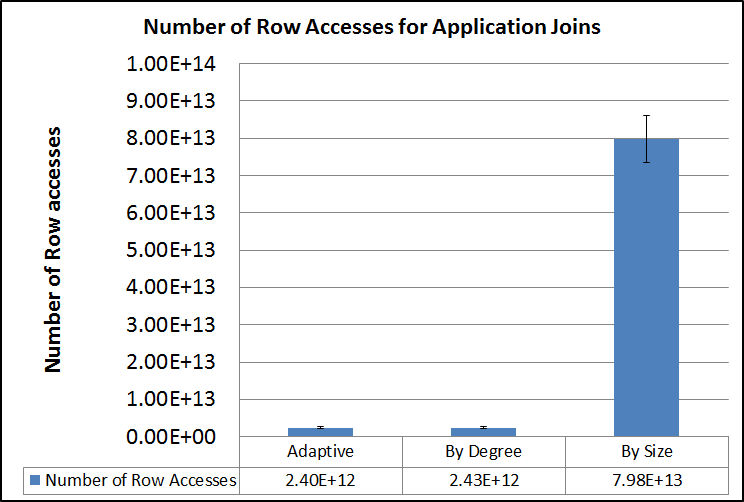
\includegraphics[width=1\columnwidth]{row-accesses.png}
\label{fig:row-accesses}}
\hfil
\subfloat[]{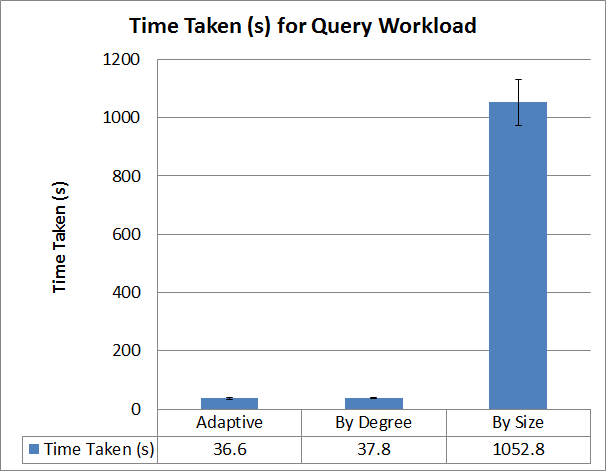
\includegraphics[width=.9\columnwidth]{time-accesses.png}
\label{fig:time-accesses}}}
\caption{\footnotesize{(a) Comparison of the number of row accesses for application-level joins when running the query workload on a dataset of size \texttt{1GB}. (b) Comparison of the time taken when running the query workload on a dataset of size \texttt{1MB}.}}
\label{fig:stats-accesses}
\end{figure*}
}

\subsection{Environment}
\label{sec:environment}
We use four nodes on the Emulab~\cite{web:emulab} network testbed for our system - one node serves as the \texttt{locator} for the SQLFire system which coordinates the data servers.  The remaining three serve as \texttt{data servers} for the tables.  SQLFire keeps the tables in memory, hence we create and populate the tables (with schema Figure~\ref{fig:schema}) with the generated rows whenever the system is restarted. The Emulab nodes have \texttt{64-bit Xeon} processor, \texttt{2 GB} of RAM and are running 64-bit version \texttt{Ubuntu 10.04}.  We, however, only allow data servers to use up to \texttt{0.5 GB} for storing tables.

\begin{figure}
\centering
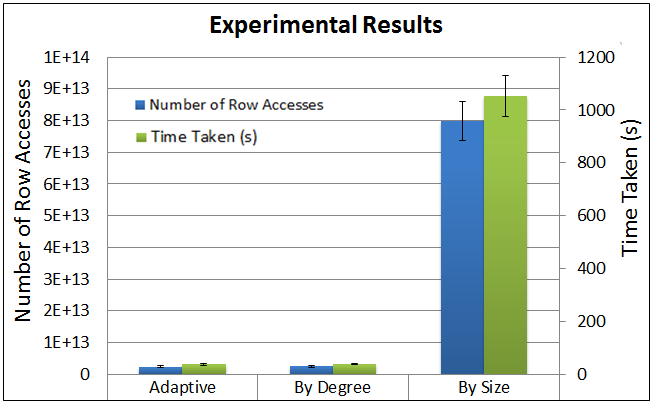
\includegraphics[width=1\columnwidth]{combined-accesses.png}
\caption{\footnotesize{Comparison of the number of row accesses for application-level joins when running the query workload on a dataset of size \texttt{1GB} and time taken to run workload on dataset of size \texttt{1MB}.}}
\label{fig:combined-accesses}
\end{figure}

\subsection{Alternative Placement Strategies}
Alternative viable methods exist for deciding the placement of data in a NewSQL system.  

\begin{itemize}
\vspace*{-9pt}
  \item \emph{Size Strategy} - A method of deciding what tables to partition on, recommended by VMWare in the documentation of SQLFire, is to choose the tables of largest size.  The data of the large tables can then be split evenly amongst the servers of a system.  According to Table \ref{tab:dataset1gb}, this would involve selecting \texttt{lineitem}, \texttt{orders}, and \texttt{partsupp} as entity group "centers" to partition on the primary keys of.  One can then use foreign key relationships to find other tables to partition and colocate with an entity center.  Any tables without foreign key relationships to the entity centers are then chosen to be replicated.
\vspace*{-18pt}
  \item \emph{Degree Strategy} - Another method is to look at the graph of parent to child relationships as in Figure \ref{fig:schema} and choose the tables with the highest degree as entity group centers to partition on the primary keys of.  This would involve selecting \texttt{part}, \texttt{supplier}, and \texttt{nation} to partition on.  One can then partition the children of these tables and colocate them with their parents.  Tables that are not a child of any center are chosen to be replicated.  This strategy is similar to the method we developed except it uses a graph with unweighted edges without consideration of the query workload.
\end{itemize}

\vspace*{-7pt} \noindent While these methods are intuitively sound, our method has the advantage of adapting to query workloads to produce optimized data placement configurations.  We compare our method against the degree and the size strategy in the following sections.
\label{sec:alternative}

\subsection{Experiment}
\label{sec:experiment}
With our experimentation, we aim to quantify and minimize both the number of row accesses performed to execute joins on non-colocated tables in a query workload and the total completion time to execute a query workload.  As of the current release of SQLFire, distributed joins involving tables or partitions that are not colocated on a server are not supported.  In such a case, it is up to the application developer to break a query that uses such joins into table fetches and an application-level join, similar to the case in most NoSQL systems.  

We thus work with this limitation by first modifying TPC-H into a purely join-based workload by stripping all the query templates of any aggregates, sorting, grouping, and non-join filter conditions.  We then write a Java client that uses JDBC to connect to our SQLFire system and sends the queries of our randomly generated TPC-H workloads.  For each query, if we are notified of a failure due to attempting to conduct a distributed join, we separate each join of the failed query into its own separate query.  We then sequentially send the new join queries to the system.  Joins on colocated tables are executed on the data servers, and those that are not colocated are further handled through an application-level join.  Application joins are conducted in a simple manner by fetching both of the tables involved and then having the application scan the entirety of one table for every row in the other table.  We keep track of the number of row accesses that an application needs to do in such application-level joins.  While this is a naive way of performing a join, we use it, as the number of row accesses involved is easily quantified through Equation \ref{eq:cost}.

\subsection{Results}
\label{sec:results}
We use the default TPC-H dataset of size 1GB with our five randomly generated workloads and the data placement configurations produced by our method, the degree strategy, and the size strategy.  The average total number of row accesses for application-level joins in each workload is shown in Figure \ref{fig:combined-accesses} and was calculated using Equation \ref{eq:cost} without actually executing the application joins.  We also measure the time taken to execute the five workloads using the same data placement configurations with executing application-level joins, but with a reduced TPC-H dataset size scaled down to 1MB.  The scaled down dataset size is necessary for our workloads to finish within reasonable amounts of time, as we stripped non-join filter conditions from the queries.  The average number of seconds to complete each workload is also shown in Figure \ref{fig:combined-accesses}.

Interestingly, deciding to partition based on a table's size resulted in a fairly suboptimal configuration for all workloads.  Partitioning based on degree, however, resulted in a configuration that was not much worse than those produced by our adaptive method. We reason that this is due to the random nature of the workload, which causes there to be an equal amount of queries representing each edge of the parent to child join graph, meaning that there is great benefit derived from simply picking nodes with high degree as partition centers.

\subsection{Adaptivity}
\label{sec:adaptivity}
Partitioning based on degree, or any static strategy, is reasonably not a good strategy for handling all kinds of query workloads.  If a query workload happens to place emphasis on a join of tables that are not colocated through the strategy, then it would be fairly detrimental and maladaptive to use the data configuration provided by the strategy.  We test this by generating another TPC-H based workload that will use a query with a join of tables not colocated by the degree strategy 75\% of the time and select from the rest of the queries the remaining 25\% of the time.  We generate 60 queries using this method, and again measure row accesses for application level joins with a \texttt{1GB} dataset and completion time of the entire workload with a \texttt{1MB} dataset.  The results for the workload are shown in Table~\ref{tab:antiDegree}.

As expected, partitioning by degree results in a poor configuration for handling the workload while our method adapts appropriately.  In fact, by focusing 75\% of the workload onto a single join, the size of the set of joins to accommodate for in the workload decreases to the point that our method can colocate all tables involved in joins.

\begin{table}
\centering
\resizebox{6cm}{!}{
    \begin{tabular}{ | c | c | c | p{5cm} |}
        \hline
        \textbf{Strategy} & \textbf{Row Accesses in App. Joins} & \textbf{Time(s)} \\ \hline
        Adaptive & 0.0 &  13\\ \hline
        By Degree & 4.563E13 & 622\\ \hline
        By Size & 1.806E14 & 2674\\
        \hline
    \end{tabular}
    }
\caption{\footnotesize{Results for query workload selected against degree
strategy.}}
\label{tab:antiDegree}
\end{table}

%\begin{figure}
%\centering
%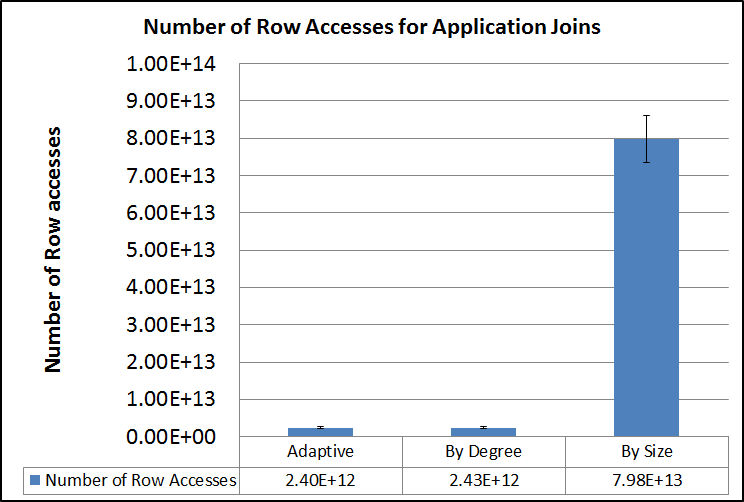
\includegraphics[scale=0.38]{row-accesses.png}
%\caption{Comparison of the number of row accesses for application-level joins when running the query workload on a dataset of size \texttt{1GB}.}
%\label{fig:row-accesses}
%\end{figure}

%\begin{figure}
%\centering
%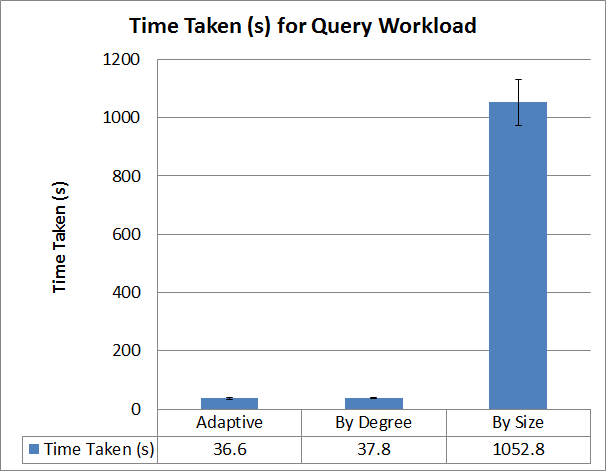
\includegraphics[scale=0.44]{time-accesses.png}
%\caption{Comparison of the time taken when running the query workload on a dataset of size \texttt{1MB}.}
%\label{fig:time-accesses}
%\end{figure}


\section{Related Work}
\label{sec:related}
We borrow many of our ideas from database literature on automatically enumerating materialized views for SQL databases (\cite{Yang:1997}, \cite{Agrawal:2000}, \cite{Phan:2008}).

In \cite{Yang:1997}, the idea of an Multiple View Processing Plan (MVPP) is used to generate optimal views. An MVPP is a directed graph that encodes the query access plan for a set of queries. For each intermediate result, a cost is calculated for storing the result as a view that involves both the cost to materialize the view and the cost to maintain the view. The authors provide a heuristic to reduce the search space of this graph. Lastly, they formulate the above problem as 0-1 integer programming.

The authors in \cite{Agrawal:2000} also provide another heuristic to decrease the exponential search space discussed above. To prune the set of candidate views further, the authors use a query optimizer to ensure that a view is part of the optimal evaluation plan for at least one query in the workload. Additionally, they use a method of view merging to get new views that do not exist in specific query but could be used to help multiple queries in the workload.

% Need one more reference in related work?
In \cite{Phan:2008}, the authors consider a setting where one is using a database cluster to evaluate OLAP-type query workloads. If we assume we are using materialized views to speed up evaluation of queries, we need an optimal query-to-server and materialied -view-to-server mapping so that the query workload execution time is minimized. To find these two mappings, the authors propose a genetic algorithm to avoid doing exhaustive search on the exponential search space. The authors show that this heuristic is only 9\% worse than exhaustive search on the TPC-H benchmark.
\section{Conclusion}
\label{sec:conclusion}
In this paper, we presented an adaptive approach to data placement in NewSQL systems, given a data model and a query workload. With a choice of how to colocate data that use partitioning and replication, we describe a method that adapts to workloads to minimize the number of distributed joins involved. Though our analysis can be generalized, we implemented our method specifically for SQLFire. We compared our adaptive approach with two other viable data placement strategies and showed that our strategy was better able to adjust to various query workloads. 
%\pagebreak
%% Bibliography
%\vspace{-1ex}
%\linespread{1.0}
%\setlength{\bibsep}{1pt}
%\footnotesize
{\small
\bibliography{local}
\bibliographystyle{abbrvnat}
}
%\appendix
\section{Appendix}
\label{sec:appendix}
For the TPC-H benchmark query generator \texttt{qgen} to generate the queries, we had to fix a minor bug in \texttt{appendix/dbgen/config.h}. Line \texttt{65} in that file specifies an incorrect format specifier (for C) in the generation of \texttt{long long} numbers i.e.,\\
\centerline{\texttt{$\#$define HUGE\_FORMAT ``\%LLd''}}\\
\noindent should change to\\
\centerline{\texttt{$\#$define HUGE\_FORMAT ``\%lld''}}

\end{document}